\documentclass[12pt,a4paper,titlepage]{article}
\usepackage[utf8]{inputenc}
\usepackage{amsmath}
\usepackage{algorithm}
\usepackage[noend]{algpseudocode}
\usepackage{amsfonts}
\usepackage{amssymb}
\usepackage{graphicx}
\usepackage{color}
\usepackage{float}
\usepackage[margin=1in]{geometry}
\author{800107 - Daniel Ng See Cheong\\
		839521 - Uzair Moolla}
\title{
	AAA Project Report\\
	\large Solving Sudoku using the backtracking algorithm
}

\graphicspath{ {images/} }

\newcommand{\todo}[1]{\textcolor{red}{\textbf{\##1\#}}}

\begin{document}
\maketitle
\newpage
\tableofcontents
\newpage
\section{Introduction}

Sudoku is a numerical based logic puzzle game. The idea is to fill in an $n\times n$ grid with numbers in a specific manner. The most commonly known grid usually consists of square blocks with 3 rows and 3 columns. These individual blocks are then arranged in a similar manner again, with 3 blocks along each row and 3 blocks along each column, producing a $9 \times 9$ matrix. An example of this described matrix can be seen in Figure  \ref{fig:Blank_Sudoku_Board}. Each individual block needs to be filled in  with one of these numbers: ${1,2,3,4,5,6,7,8,9}$.
\\
\\
The rules for filling in the $9 \times 9$ sudoku grid are as follows:
\begin{itemize}
\item[•] Within each $3 \times 3 $ block we can only have a single occurrence of each number.
\item[•] Along each row of $9$ blocks we can only have a single occurrence of each number.
\item[•] Along each column of $9$ blocks we can only have a single occurrence of each number.
\end{itemize}

\noindent
An example of a Sudoku Puzzle completed using the rules stated above can be seen in Figure \ref{fig:Complete_Sudoku_Board}.

\begin{figure}[H]
\centering
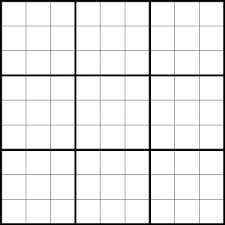
\includegraphics[scale=0.5]{Blank_Sudoku_Board}
\caption{Sample of a $9\times9$ Blank Sudoku Board}
\label{fig:Blank_Sudoku_Board}
\end{figure}
%-------------------------------------------------------%
\begin{figure}[H]
\centering
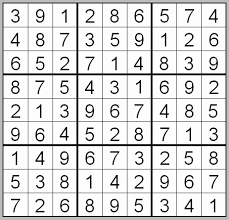
\includegraphics[scale=0.5]{Complete_Sudoku_Board}
\caption{Sample of a $9\times9$ Completed Sudoku Board}
\label{fig:Complete_Sudoku_Board}
\end{figure}
%------------------------------------------------------%

\noindent
Solving sudoku puzzles are a fun exercise for many. However we would like to find a suitable algorithm which can be used to solve sudoku puzzles correctly as well as efficiently. There are various possible methods which can be used to solve sudoku puzzles. We will be focussing on the \emph{Backtracking Algorithm} in our experiments.
\\

\newpage
\section{Aims}

We are going to use the backtracking algorithm to solve sudoku puzzles of size $9\times 9$. We will attempt to solve these sudoku puzzles accurately and in as little time as possible. Once we have the algorithm working correctly we will perform both theoretical as well as empirical analysis on it. We aim to find the best and worst case complexities of the algorithm being used. These results will be obtained through both methods of analyses (empirical as well as theoretical) and correlations between the results will be obtained.
\\
\\
We will create a database of unsolved puzzles using a random puzzle generator. These generated puzzles will either have a unique solution, multiple solutions or no solution. These puzzles will be used for all analysis done. 
\\

\section{Summary of Theory}

\subsection{Backtracking Algorithm}

In general backtracking algorithms are mainly used to solve NP-complete computational problems. Simply put, the backtracking algorithm starts with the selection of one possible move out of all available moves and will try solving the problem with the selected move. If the selected move allows us to find a correct final solution to the problem, the solution is given as an output (it is printed out). However, if the selected move does not lead to a correct final solution to the problem, we backtrack. The backtracking is done to the point where the move was selected and we then choose an alternative move at this point. This process is repeated until the correct solution to the problem is found. If none of the available moves work in finding the correct solution to the problem it is sufficient to say there is no solution to the problem.
\\
Recursion is the most appropriate method to implement this type of algorithm.


\section{Pseudo code}

\begin{algorithm}[H]
\caption{Check if  a Move is Valid}
\begin{algorithmic}[1]

\Function{validMove}{number , row, column}
\\
Where:
\\
\textit{number} is the number to be inserted
\\
\textit{row} is the row of current position
\\
\textit{col} is the column of the current position
\\
\textit{n} is the length of the square matrix representing the sudoku puzzle grid 
\\
\textit{board} is the $n \times n$ square matrix representing the sudoku puzzle grid 
\\

	\For{i from 1 to n}
		\If{number is equal to board[row][i]}	
			\State return false
		\EndIf
	\EndFor 	

	\For{i from 1 to n}
		\If{number is equal to board[i][col]}	
			\State return false
		\EndIf
	\EndFor	
	
	
	\\
	\\
	initialise rowmin to $ \dfrac{row}{blocksize} \times blocksize $
	\\
	\\	
	initialise colmin to $ \dfrac{column}{blocksize} \times blocksize $
	\\
	\\		
	initialise rowmax to (rowmin + blocksize)
	\\		
	initialise colmax to (colmin + blocksize)	
	\\
	
	\For{i from rowmin to rowmax }
		\For{j from colmin to colmax}  	 
			\If{number = board[i][j]}
	   			\State return false
	 		\EndIf       
  		\EndFor
  	\EndFor
	\State return true
\EndFunction
\end{algorithmic}
\end{algorithm}

%---------------------------------------------------------------------

\begin{algorithm}[H]
\caption{Check if a Position is Open}
\begin{algorithmic}[1]
\Function{openPosition}{}
\\
\textit{n} is the length of the square matrix representing the sudoku puzzle grid
\\
\textit{board} is the $n \times n$ square matrix representing the sudoku puzzle grid 
\\ 
\State initialise temp to be an array of length 2
  
	\For{i from 1 to n}
		\For{j from 1 to n}  	 
			\If{board[i][j] is empty}
				\State temp[0] = i
				\State temp[1] = j
				\State return temp 
			\EndIf       
		\EndFor
	\EndFor
	\State  return NULL
\EndFunction

\end{algorithmic}
\end{algorithm}

%----------------------------------------------------------------

\begin{algorithm}[H]
\caption{Backtracking}
\begin{algorithmic}[1]
\Function{solve}{}
\\
\textit{n} is the length of the square matrix representing the sudoku puzzle grid 
\\
\textit{board} is the $n \times n$ square matrix representing the sudoku puzzle grid
\\
\textit{openPosition(),validMove(i,row,col)} are the functions described above in Algorithm 1 and Algorithm 2 respectively.
\\ 
	\State initialise row and col; 
	\State initialise temp to openPosition();	

	\If{temp is not NULL} 
		\State row = temp[0];
		\State col = temp[1];
  	\Else
		\State return true
	\EndIf  
	
	\For{i from 1 to n}
		\If{validMove(i,row,col) is true}
			\State board[row][col]=i;
       		\If{solve() is true}
       			\State return true;
       		\EndIf       
			\State set board[row][col] to be empty;
		\EndIf
	\EndFor
	\State  return false;
\EndFunction

\end{algorithmic}
\end{algorithm}

\section{Theoretical Analysis }

Theoretical analysis will be done for each of the algorithms listed above. Even though the first two algorithms are used in the Backtracking Algorithm (ie Solve calls validMove as well as openPosition) we will be calculating their complexities individually and thereafter include them in the complexity calculation of the Backtracking Algorithm. We are able to do this as the aim of this experiment is to find the complexity of the Backtracking Algorithm being used to solve a sudoku puzzle.

\subsection{Algorithm 1: validMove}
 
The algorithm validMove is given the number to be inserted as well as the row and column where it will be inserted in the sudoku puzzle. It then runs through the puzzle being filled in and checks if the three rules listed above are not violated by the insertion of the particular number at that position.
\\
\\
For the theoretical analysis of this algorithm we will use comparisons as the basic operation. There are two main segments in this algorithm, the first simply checks if  the number to be inserted in the puzzle already exists in the row or column of the block wherein we want to insert the number. The second segment checks if the number to be inserted exists in the sub-block of the sudoku puzzle as mentioned in the rules of sudoku.
\\
\\

\subsubsection{Best Case}

In the best case this algorithm would exit at line 11. This would happen when the number in position [r][1] is the same as the number to be inserted into row r. This means the time complexity of Algorithm 1 in the best case is $O(1)$.

\subsubsection{Worst case}

In the worst case the algorithm would exit at line 27. This would happen when all the rules are valid and the number can be inserted into the position being checked. Therefore the time complexity of this algorithm in the worst case is $O(n)$ for a sudoku board of size $n$.

\subsection{Algorithm 2: openPosition}

The algorithm openPosition does not require any inputs. It then runs through the sudoku puzzle being filled in and searches for blocks (positions) which are empty in the puzzle being filled in. The empty blocks are represented by 0 in the puzzle.
\\
\\
For the theoretical analysis of this algorithm we will use comparisons as the basic operation. This algorithm simply loops through all positions in the sudoku puzzle searching for an empty block wherein we can fill a number according to the rules of sudoku. 

\subsubsection{Best Case}

In the best case this algorithm would exit in line 11. The best case complexity will occur when the open position is the first block searched in the puzzle i.e. position [1][1] in the matrix. Therefore the complexity of this algorithm in the best case is $O(1)$.

\subsubsection{Worst Case}

In the worst case the algorithm has two possibilities. The first is if the board only has one last open position i.e. [n][n] is open for a board of size $n$. The second is if there are no open positions left on the board. In both cases the complexity is $O(n^{2})$. Thus the time complexity of this algorithm in the worst case is $O(n^{2})$ for a sudoku board of size $n$.

\newpage
\subsection{Algorithm 3: Solve}

The algorithm Solve does not take in any input. It is the backtracking algorithm we are using to solve sudoku puzzles. The algorithm initialises row and column and finds an open position on the board using the openPosition algorithm. It then tries to fill in a number using the validMove algorithm. If this does not work it backtracks and reattempts to solve the sudoku puzzle. This process is repeated until a final unique solution is found.

\subsubsection{Best Case}

In the best case this algorithm would exit in line 12. The best case complexity will occur when there are no open positions in the puzzle. This implies that the puzzle is already solved. For this we need to take into account the complexity of openPosition in this situation. The board in this situation would be a completely full. Therefore the complexity of this algorithm in the best case is $O(n^{2})$ for a sudoku board of size $n$.


\subsubsection{Worst Case}

In the worst case The algorithm would have to use the algorithms openPosition as well as validMove on every choice made. We also have to consider the recursion which takes place in line 16. Taking all this into account we see that the algorithm would have a worst case complexity of $O(n^{m})$ where m is the number of blank or empty blocks in the initial sudoku puzzle of size $n \times n$. The reason for this is the recursive nature of the backtracking algorithm. It also represents every possible permutation of the puzzle.


\section{Experimental Methodology}

For our experiments we have written code that will generate a sudoku puzzle of a given size $n$ and fill in $f$ random positions within the puzzle with random numbers between $1$ and $n$. The number of positions filled in ($f$) can be changed as it is taken as an input in the generator algorithm. We will then run our backtracking algorithm \emph{Solve} on this generated puzzle and the output will either be the solution to the puzzle or, if none exists, then the algorithm will print out "No Solution". This process will be repeated 1000 times for each $f$ by the random puzzle generator. These 1000 iterations will each be timed and then averaged to produce a final time for solving a puzzle where the number of filled in blocks is $f$. The variable $f$ will always be between $1$ and $81$ in our experiments.

The reason for testing our algorithm in this mannor is that we can determine $m$, the number of empty or blank positions in the given puzzle at every iteration.  

\section{Presentation of results}

%-------------------------------------------------------%
\begin{figure}[H]
\centering
\includegraphics[width = \textwidth]{graph1}
\caption{Results of empirical analysis}
\label{fig:graph1}
\end{figure}
%------------------------------------------------------%

\section{Interpretation of results}

In Figure \ref{fig:graph1} each plotted line represents a single test. Each test was performed as explained in our Experimental Methodology. From the results we see that for $f$ between 1 and 10 the sudoku puzzle is solved in a relatively short amount of time. A possible reason for this is that as the puzzles are randomly generated there may be multiple solutions to each puzzle.
\\
\\
Also in Figure \ref{fig:graph1} We see that for $f$ between 10 and 30 solving the sudoku puzzle takes the greatest amount of time. The reason for this is that, as some mathematicians theorise, a sudoku puzzle has a unique solution when a certain number of blocks have been filled in. This would imply that at these points the algorithm searches for the unique solution backtracking the most. This would happen often as the backtracking would occur regardless of whether a unique solution is found or not. This would be the worst case time complexity of our algorithm. 
\\
\\
The best case complexity occurs when $f$ is greater than 45. The reason for this is that the number of open positions start decreasing at this point and thus the algorithm has much less work to do.    

\newpage
\section{Conclusion}

We set out to determine the time complexity of the backtracking algorithm we designed to solve a sudoku puzzle of size $ 9 \times 9$. The algorithm does find solutions to every solvable sudoku puzzle given to it as an input. We have also been able to determine the best as well as the worst case complexities both theoretically and empirically. The complexities we have obtained through empirical analysis do align with those obtained in theoretical analysis. All in all this research has been a success as we have been successful in completing the aims as set out when we began this project.

\section{References}


\end{document}